This chapter provides a brief summary of the Dispersive Optical Model.
A few motivating concepts and definitions, sourced from the extensive treatments of \cite{MahzoonPhDThesis, MBTE},
are followed by an explicit parameterization of the optical potential used for the DOM fits of Chapter \ref{DOMResults}.
For all sectors of experimental data used in said fits, the formulae connecting the optical potential
to the scattering data are given. For detail on the development of the DOM formalism, the seminal
work of Mahaux and Sartor \cite{Mahaux1991} and a recent review \cite{Dickhoff2018} are recommended.
The goal here is not to provide the complete underpinnings of the theory, which are available in
numerous sources elsewhere, but to discuss how the terms of the potential are sensitive
to different sectors of experimental data.
In addition, several computational improvements to our implementation of the DOM, important for
expanding the reach of the fully non-local DOM of \cite{MahzoonPhDThesis} to all even-even systems,
are pointed out. In all cases, the notation used conforms to \cite{MBTE}, which also provides an
introduction to second quantization and historical background for relevant many-body concepts.

\section{The Single-Particle Propagator}
The central project of the Dispersive Optical Model (like any optical model) is
to understand how nucleons move about in a nuclear many-body system, as parameterized by an optical
potential.
Specifically, we wish to know
how a nucleon with energy $E$ and quantum numbers $\alpha$
(position, momentum, spin, isospin, etc.) at time $t_{0}$ will be measured at a
later time $t$ with quantum numbers $\beta$ after interaction with the
potential. Given a
Hamiltonian that models this interaction, the Schr\"odinger equation
relates the Hamiltonian to the time evolution of this state:

\begin{equation} \label{SchrodingerEquation}
    i\hbar\frac{\partial}{\partial t}\ket{\alpha, t_{0};t} = H\ket{\alpha,
    t_{0}; t}
\end{equation}

where $\ket{\alpha, t_{0},t}$ is the state at time $t$, given an initial state
$\ket{\alpha, t_{0}}$. Simple substitution into \label{SchrodingerEquation} shows
that the initial state propagates in time according to:

\begin{equation}
    \ket{\alpha, t_{0}, t} = e^{-\frac{i}{\hbar}H(t-t_{0})}\ket{\alpha, t_{0}}
\end{equation}

In position space, the wavefunction of the particle at time $t$, $\psi(\bm{r},t)$,
is the sum of over all contributions from the propagation of the initial state, a direct application of
Huygens principle:

\begin{equation} \label{PropagatorDerivation}
    \begin{split}
        \psi(\bm{r},t) & = \braket{r|\alpha, t_{0}; t}\\
        & = \int d\bm{r}'
        \braket{\bm{r}|e^{-\frac{i}{\hbar}H(t-t_{0})}|\bm{r'}}\braket{\bm{r'}|\alpha,t_{0}}
    \end{split}
\end{equation}

\noindent
where we have inserted the $\bm{r'}$ basis on the right side of the equation.
The integrand of Eq. \ref{PropagatorDerivation} is referred to as the ``single-particle propagator'' 
(denoted $G(r, r'; t-t_{0})$ in the time domain),
as it determines how the wavefunction of a single particle
propagates over time. Crudely speaking, the propagator can be interpreted as the chance that a given
initial state will evolve into a final state according to the wave equation.

To conduct practical scattering calculations, the energy-domain representation of the progapator
may be more useful than the time-domain representation. Applying a Fourier Transform to the propagator
(and omitting the intermediate algebraic steps) gives us this representation, which brings the mathematical
structure of the propagator into focus:

\begin{equation} \label{PropagatorFT}
    \begin{split}
        G(\bm{r},\bm{r'};E) & = \int_{-\infty}^{\infty}d(t-t')e^\frac{i}{\hbar}E(t-t')G(\bm{r},\bm{r'}; t-t')\\
        & = \braket{0|a_{\bm{r}}\frac{1}{E-H+i\eta}a^{\dagger}_{\bm{r'}}|0}\\
        & = \braket{\bm{r} | \frac{1}{E-H+i\eta} | \bm{r'}}
    \end{split}
\end{equation}

\noindent
where $a_{\bm{r}}$ and $a^{\dagger}_{\bm{r}}$ represent the particle removal and
addition operators in
the second-quantization picture, respectively, and $\ket{0}$ is the vacuum state.
Equation \ref{PropagatorFT} contains the same information as Eq. \ref{PropagatorDerivation}: that
the wavefunction $\psi(r)$ is the sum of the weighted contributions from all $r'$ and the weights
are determined by the difference between the energy $E$ and the evaluation of $H$ on each of the $r'$
contributions. Of course, we need not privilege $\bm{r}$-space; $G$ can be written using any
suitable single-particle basis. For example, the momentum-space representation for a spinless,
non-interacting free particle of mass $m$ and momentum $\bm{k}$ reads:

\begin{equation} \label{PropagatorKSpace}
    G^{0}(\bm{k}, \bm{k'}; E) = \delta(\bm{k}-\bm{k'})\frac{1}{E-\frac{\hbar^{2}k^{2}}{2m} + i\eta}
\end{equation}

\noindent
If the independent-particle model was exact and the mean-field potential could be perfectly known,
calculating the propagation of nucleons through the nucleus would as simple as calculating
single-particle scattering off a potential well. Such a calculation involves little more than
a matrix inversion of the Hamiltonian in the denominator of Eq. \ref{PropagatorFT}.
Real nucleon-nucleus scattering involves the possibility of excitations in the nucleus from the 
incident
nucleon so that the wavefunction of the compound system is very different from the ground state of
the nucleus. The single-particle propagator must include these possibilities as well.
The propagator from the $\ket{\alpha}$ state at time $t$ to the state $\ket{\beta}$ at a later time
$t'$ is:

\begin{equation} \label{ManyBodySPPropagator}
    G(\alpha, \beta; t, t') =
    -\frac{i}{\hbar}\braket{\Psi^{N}_{0}|\mathcal{T}[a_{\alpha_{H}}(t)a^{\dagger}_{\beta_{H}}(t')]|\Psi^{N}_{0}}
\end{equation}

\noindent
Here, $\ket{\Psi^{N}_{0}}$ is the normalized Heisenberg ground state for the N-particle system with
eigenvalue $E^{N}_{0}$:

\begin{equation} \label{NParticleGroundState}
    \hat{H}\ket{\Psi^{N}_{0}} = E^{N}_{0}\ket{\Psi^{N}_{0}}
\end{equation}

The time-ordering operator $\mathcal{T}$\footnote{
    The time-ordering operator $T$ is defined as:
    \begin{equation*}
        \mathcal{T}[a_{\alpha_{H}}(t)a^{\dagger}_{\beta_{H}}(t')]=\theta(t-t')a_{\alpha_{H}}(t)a^{\dagger}_{\beta_{H}}(t')
        -\theta(t'-t)a^{\dagger}_{\beta_{H}}(t')a_{\alpha_{H}}(t)
    \end{equation*}
} ensures that operators with later time appear to the left
of operators with earlier time, important for the perturbative treatment to follow.
In short, this expression includes contributions from both particle propagation, already seen for 
the particle
propagation in vacuum of Eq. \ref{PropagatorDerivation}, and hole propagation, new behavior only
relevant for a many-particle system capable of excitation. We can expand Eq.
\ref{ManyBodySPPropagator} and once again apply a Fourier transform to make
interpretation easier:

\begin{equation} \label{LehmannRepresentation}
    \begin{split}
        G(\alpha,\beta;E) & =
        \int_{-\infty}^{\infty}d(t-t')e^{\frac{i}{\hbar}E(t-t')}G(\alpha,\beta;t-t')\\
        & = \sum_m
        \frac{\braket{\Psi^{N}_{0}|a_{\alpha}|\Psi^{N+1}_{m}}\braket{\Psi^{N+1}_{m}|a^{\dagger}_{\beta}|\Psi^{N}_{0}}}
        {E-(E^{N+1}_{m}-E^{N}_{0})+i\eta} +
        \frac{\braket{\Psi^{N}_{0}|a_{\beta}|\Psi^{N-1}_{n}}\braket{\Psi^{N-1}_{n}|a^{\dagger}_{\alpha}|\Psi^{N}_{0}}}
        {E-(E^{N}_{0}-E^{N-1}_{n})+i\eta}\\
        & =
        \braket{\Psi^{N}_{0}|a_{\alpha}\frac{1}{E-(\hat{H}-E_{0}^{N})+i\eta}a^{\dagger}_{\beta}|\Psi^{N}_{0}} +
        \braket{\Psi^{N}_{0}|a^{\dagger}_{\beta}\frac{1}{E-(E^{N}_{0}-\hat{H})-i\eta}a_{\alpha}|\Psi^{N}_{0}}
    \end{split}
\end{equation}

\noindent
Here, $\Psi^{N\pm1}_{m(n)}$ are the normalized Heisenberg states for the N\pm1 particle 
systems. The $\Psi^{N+1}_{m}$ have eigenvalues $E^{N+1}_{m}$ and the $\Psi^{N-1}_{n}$ have 
eigenvalues $E^{N-1}_{n}$:

\begin{equation}
    \begin{align}
        \hat{H}\ket{\Psi^{N+1}_{m}} & = E^{N+1}_{m}\ket{\Psi^{N+1}_{m}}\\
        \hat{H}\ket{\Psi^{N-1}_{n}} & = E^{N-1}_{n}\ket{\Psi^{N-1}_{n}}
    \end{align}
\end{equation}

The second line of Eq. \ref{LehmannRepresentation} was propounded by Lehmann \cite{Lehmann1954} and
is referred to as the ``Lehmann representation''. To reach the third line, the complete set of
$\Psi^{N+1}_{m}$ and $\Psi^{N-1}_{n}$ have been removed from the first and second addends of line
two, respectively. The particle and hole contributions to the propagator are neatly separated and
each possess the relevant energy weighting in the denominator sandwiched between the fermion 
creation and annihilation operators. Neither the ground-state wavefunction of the correlated
many-body system $\Psi^{N}_{0}$ or the full Hamiltonian $\hat{H}$ are known at this stage, but they
are amenable to a perturbation expansion, the subject of the next section.

\subsection{Pertubation Expansion: The Dyson Equation}
The full single-particle propagator $G$ of the previous section can be calculated via perturbation
expansion by starting with a non-interacting (unperturbed) propagator $G_{0}$ and adding interaction 
terms, $\hat{V}$, that bring $G_{0}$ closer to the real $G$. This expansion requires a change from
the Heisenberg picture of the previous section to the Interaction picture\footnote{Operators in the
    Interaction picture are related to those in the Schr\"odinger picture by:
    \begin{equation*}
        O_{I}(t) = e^{\frac{i}{\hbar}\hat{H}_{0}t}O_{S}e^{\frac{-i}{\hbar}\hat{H}_{0}t}
    \end{equation*}
    Appendix A of \cite{MBTE} provides a complete description of these different quantum-mechanical
pictures.}. First, the full Hamiltonian $H$ is broken up into the non-interacting and interacting
parts:

\begin{equation}
    \hat{H} = \hat{H_{0}}+\hat{H}_{1}
\end{equation}

where $\hat{H_{0}}$ contains the kinetic energy operator $\hat{T}$ and possibly a one-body auxiliary
potential $\hat{U}$, and $\hat{H_{1}}$ collects all residual interactions (the hard part of the
problem). Broken up in this way, the non-interacting propagator reads:

\begin{equation}
    G^{(0)}(\alpha, \beta; t-t') =
    -\frac{i}{\hbar}\braket{\Phi^{A}_{0}|
    \mathcal{T}[a_{\alphaI}(t)a^{\dagger}_{\betaI}(t')]|\Phi^{A}_{0}}
\end{equation}

where the fully-correlated many-body ground state $\Psi^{A}_{0}$ has been replaced by
$\Psi^{A}_{0}$, the uncorrelated ground-state associated with $H_{0}$. Through algebraic
manipulation and application of Wick's theorem, the \textit{full} propagator, including the
contribution from the interactions buried in $\hat{H_{1}}$, is:

\begin{equation}
    G(\alpha, \beta; t-t') =
    -\frac{i}{\hbar}\sum^{\infty}_{n}(\frac{i}{\hbar})^{n}
    \frac{1}{n!}\int dt_{1} \int dt_{2} \cdots \int dt_{n} \times
    \braket{\Phi^{A}_{0}|
    \mathcal{T}[\hat{H}_{1}(t_{1})
    \hat{H}_{1}(t_{2}) \cdots \hat{H}_{1}(t_{n})a_{\alphaI}(t)a^{\dagger}_{\betaI}(t')]|\Phi^{A}_{0}}
    _{connected}
\end{equation}


\begin{equation}
    G(\alpha, \beta; t-t') =
    -\frac{i}{\hbar}\sum^{\infty}_{n}(\frac{i}{\hbar})^{n}
    \frac{1}{n!}\int dt_{1} \int dt_{2} \cdots \int dt_{n} \times
    \braket{\Phi^{A}_{0}|
    \mathcal{T}[\hat{H}_{1}(t_{1})
    \hat{H}_{1}(t_{2}) \cdots \hat{H}_{1}(t_{n})a_{\alphaI}(t)a^{\dagger}_{\betaI}(t')]|\Phi^{A}_{0}}
    _{connected}
\end{equation}

Physically speaking, the full propagator is an expectation value of 
an infinite sum of $\hat{H_{1}}$ applied to the non-interacting ground state. The
non-interacting ground state is modified by each interaction and thus all the many-body correlations
of $\Psi^{N}_{0}$ are encoded by the repeated operation of $\hat{H_{1}}$. The application of Wick's
theorem removes a large number of To compute this sum, only 
fully-connected Feynman diagrams should be used, as all non-connected diagrams appear on both the  The subscript
``connected'' shows that only connected Feynman diagram

\begin{figure}
    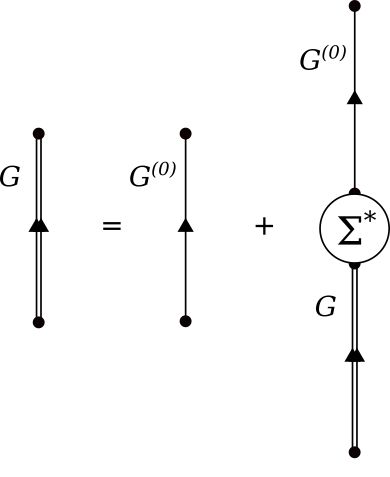
\includegraphics[scale=0.35]{figures/DysonEquation.png}
    \caption{The Dyson Equation in diagrammatic form}
    \label{DysonEquation}
\end{figure}

The Hartree-Fock potential, the default starting place for a mean-field potential,
has no energy dependence and thus cannot accommodate 

\subsection{The Dispersion Relation}
Subtracted dispersion relation.

\section{Connection to Experimental Observables}

\subsection{Elastic and inelastic nucleon scattering}
For nucleon-nucleus scattering, the scattering amplitude can be directly calculated using the
reducible self-energy:

\begin{equation}
    f_{m'_{s},m_{s}}(\theta,\phi) =
    -\frac{4m\pi^{2}}{\hbar^{2}}\braket{\boldmath{k}'m'_{s}|\Sigma(E)|\boldmath{k}m_{s}}
\end{equation}

\noindent
where $\boldmath{k}m_{s}$ are the wave vector and spin quantum number of the incident nucleon and
$\boldmath{k'}m'_{s}$ are for the exiting nucleon. The matrix structure of the right side can be
split into spin-independent and spin-dependent portions $\mathcal{F}$ and $\mathcal{G}$:

\begin{equation}
    \begin{split}
    f(\theta,\phi) & = \mathcal{F}(\theta)I + \sigma\cdot\boldmath{\hat{n}}\mathcal{G}(\theta)\\
    & = \frac{1}{2ik}\sum_{l=0}^{\infty}\left[(l+1)e^{2i\delta_{l+} - 1} +
    l\left(e^{2i\delta_{l-}}-1\right)\right]P_{l}(cos\theta) +
    \sigma\cdot\boldmath{\hat{n}}\left[\frac{sin\theta}{2k}\sum_{l=1}^{\infty}[e^{2i\delta_{l+}}-e^{2i\delta_{l-}}]P'_{l}(cos\theta)\right]
    \end{split}
\end{equation}
\noindent
where $P_{l}$

The phase shift (equivalently, the S-matrix elements) for each partial wave can be directly from the reducible self-energy:
\begin{equation}
    \begin{split}
        e^{2i\delta_{lj}} & \equiv \braket{k|\mathcal{S}_{lj}(E)|k}\\
        & = 1 - 2\pi i \left(\frac{mk}{\hbar^{2}}\right) \braket{k|\Sigma_{lj}(E)|j}
    \end{split}
\end{equation}
\noindent
where $k$ is the center-of-mass momentum of the nucleon, $m$ is the nucleon mass, and $E$ is the
center-of-mass energy. 
\subsection{Bound-state properties}

\section{Parameterization of the Potential}

To parameterize the DOM's optical potential, we rely on standard functional
forms common in nuclear theory calculations.

The real part of the potential is comprised of a Hartree-Fock component and
a spin-orbit component (plus a Coulomb term if the projectile is a proton).
The Hartree-Fock component $V_{HF}$ has two subcomponents:

\begin{equation}
    V_{HF}(r,r') = V_{vol}(r,r') + V_{WB}(r)
\end{equation}

The non-local Hartree-Fock volume term $V_{vol}(r,r')$, is defined as
a Woods-Saxon form coupled to a Gaussian non-locality:

\begin{equation}
    V_{vol}(r,r') =
    \dfrac{-V}{1+e^{(r-R)/a}}\cdot\dfrac{1}{\pi^{\frac{3}{2}}\beta^{3}}
    \exp{\frac{|r-r'|^{2}}{\beta^{2}}}
\end{equation}

where $V$, $R$, and $a$ are the depth, radius, and diffuseness of the HF potential,
and $beta$ is the extent of the non-locality. The local Hartree-Fock wine-bottle
term $V_{wb}(r)$, named for resemblence to the dimple at the bottom of a wine
bottle, is defined as a Gaussian centered at the nuclear origin:

\begin{equation}
    V_{wb}(r) = V\exp{\frac{r^{2}}{\sigma^{2}}}
\end{equation}

The real spin-orbit component $V_{so}$
is defined using a derivative-Woods-Saxon shape to
accommodate the expectation that the spin-orbit coupling is strongest near the
nuclear surface:

\begin{equation}
    V_{so}(r,r') =
    \frac{d}{dr} \frac{-V}{1+e^{\frac{(r-R)}{a}}}\cdot\frac{1}{\pi^{\frac{3}{2}}\beta^{3}} \exp{\frac{|r-r'|^{2}}{\beta^{2}}}
\end{equation}

The imaginary part of the potential is comprised of independent surface and volume terms
both above and below the Fermi surface, plus an imaginary spin-orbit term:

\begin{equation}
    V_{HF}(r,r') = V_{vol}(r,r') + V_{WB}(r)
\end{equation}

The occupation number of nucleons with quantum numbers $\alpha$ can be
calculated directly from the imaginary component of the single-particle
propagator:

\begin{eqnarray}
    n(\alpha)
    & = & \braket{\Psi^{N}_{0}|a^{\dagger}_{\alpha}a_{\alpha}|\Psi^{N}_{0}}\\
    & = & \sum_{n}|\braket{\Psi^{N-1}_{n}|a_{\alpha}|\Psi^{N}_{0}}|^{2}\\
    & = & \int_{-\infty}^{\epsilon_{F}^{-}} dE
\sum_{n}|\braket{\Psi^{N-1}_{n}|a_{\alpha}|\Psi^{N}_{0}}|^{2}
\delta(E-(E^{N}_{0}-E^{N-1}_{n}))\\
& = & \int_{-\infty}^{\epsilon_{F}^{-}} dE \frac{1}{\pi}\operatorname{Im}G(\alpha,\alpha;E)
\end{eqnarray}


For nuclei with open subshells (e.g., the $\upnu$ 0\dFive in $^{18}$O and
$\upnu$ 0\fFive in $^{58}$Ni), an additional
pairing parameter $\Delta$ was added to
account for these subshells' fractional occupatio $n_{\pm}$ of the open subshells. due to pairing
effects. This parameter splits partially-occupied subshells (e.g., the $\upnu$\dFive
for \oEight) into upper and lower sublevels with energies $E_{\pm}$:

\begin{equation}
    E_{\pm} = \mu \pm ((\epsilon_{F}-\mu)^{2} + \Delta^{2})^{frac{1}{2}}
\end{equation}

where $\mu$ is the energy of the open subshell before pairing is considered and
$\epsilon_{F}$ is the Fermi
energy. The magnitude of $\Delta$ corresponds to the energy difference between
adding/removing a nucleon to/from that subshell. The subshell's particle
capacity is split between the upper and lower sublevels, and only the :

\begin{equation}
    n_{\pm} = \frac{1}{2}\left( 1-\frac{\chi}{E_{\pm}}\right)
\end{equation}

where $\chi = |E_{\pm}-\mu| - (\epsilon_{F} - \mu)$. Only occupation in the
lower sublevel is counted toward the total particle number. For each open-shell
nucleus with nucleon numbers $N, Z$ , the pairing gap $\Delta$ was fixed according to:

\begin{equation}
    \Delta(N,Z) = \frac{1}{4}\left(B(N-2,Z)-3B(N-1,Z) + 3B(N,Z)-B(N+1,Z)\right)
\end{equation}

where $B(N,Z)$ is the nuclear binding energy.

The Dispersive Optical Model (DOM) is a phenomenological framework useful for 
extracting information about nuclear properties and structure from experimental
data.

The fundamental object of interest in the DOM is the \Gls{optical potential},
which is identified as the \Gls{nucleon self-energy}. This potential represents
the nuclear environment experienced
by a nucleon as it traverses the nucleus being represented. In general, the
potential is both non-local and complex, possessing both real (flux-conserving)
and imaginary (flux-removing) parts. The functions used to parameterize the optical potential
are selected to conform with general physical intuition about the nuclear
many-body problem and past experience with optical potentials throughout the
field. For example, the most important term, the Hartree-Fock (HF) potential
that binds the nucleus together, is defined by a classic Woods-Saxon form to
which non-locality has been added: [insert volume term formula]. The imaginary
potential is separated into a Woods-Saxon volume component and a
Woods-Saxon-derivative surface component. Each of these subcomponents has
a non-linear energy dependence reflecting our expectation that surface-like
behaviors should arise around 10-20 MeV and volume-like behavior should dominate
above 50 MeV, with a mixture of the two in the intermediate region.

Beyond these basic considerations, several additional features make the 
DOM a useful tool. First is the enforcement of a
dispersion relation (the Kramers-Kronig relations) between the real and imaginary
halves of the potential, ensuring that the potential is causal (i.e., the
time-ordering of the operator representation of the self-energy is maintained).

\section{Computational Improvements}
As with any high-dimensional optimization problem, the fitter must be vigilant
against the overfitting of data. In practice, this requires:

parsimony with the number of parameters used in the model

common-sense checking "under the hood" of the optimization to verify that
parameter values make sense given the assumptions that undergird the model

understanding of what the value function is (that is, the function being
minimized/maximized) and whether it needs to be changed

cross-correlation between parameters to understand the relationship between
parameters and the effect that each has on predictions made using the model

TCS affected by HF parameters, spin orbit, imaginary above
RCS affected by imaginary above, HF parameters
ECS affected by HF parameters, spin orbit, imaginary above
APower affected by HF parameters, spin orbit,  imaginary above
Charge Density affected by HF parameters, imaginary below
Levels affected by HF parameters, spin orbit,
Spectral functions affected by HF parameters, imaginary below
RMSRadii affected by HF parameters, imaginary below

Physical intuition about scattering data:
- the low-angle ECS/APower data are sensitive to the imaginary strength above
the Fermi surface. The high-angle ECS/APower data are sensitive to the imaginary
strength below the Fermi surface, with the highest angles of elastic scattering
probing the imaginary strength deepest in the core (see high-energy, high-angle
data in Pb)
- the NM correction to the imaginary volume strength is required in all cases to
have the very high/very low energy imaginary strength have the correct trend
(linearly increasing above 100 MeV above, decreasing to 0 below 100 MeV below).
Seen in spectral functions and total cross section data at high energies, where
the pion production channel enters the picture as it goes from virtual->real
- the general trend of the elastic scattering data (not wiggles, but averaged
over wiggles) depends on the imaginary strength at the given energy. If the
minima in the elastic cross sections are too sharp/deep, the imaginary strength
is too large at that energy
- the spin-orbit strength has dramatic effects on the total cross section at low
energies ($<$20 MeV)
- above the Fermi surface, the imaginary strength is dominated by surface from
0-50 MeV and by volume from 50 MeV up. Below the Fermi surface, the surface
imaginary strength is dependent on A; for low A, where the level density is very
low below the Fermi surface and there's almost no contribution from high LJ
levels, there is virtually no surface imaginary strength below (cf. with charge
density distribution tail, at the surface of the nucleus). As A increases, 
imaginary surface strength below increases gradually but never reaches the
imaginary surface strength above. A consequence of the asymmetry of the
operators that contribute: below 0 MeV, the removal operator LJs
must recouple to the ground state, so high LJ operators have virtually no
contribution; above 0 MeV, addition operators can have arbitrary LJs because
free scattering is possible, adding significantly to the collective strength and
thus is imaginary strength peaked at the surface in the 20-30 MeV range (giant
dipole resonance, for example, surface phonons).

\subsection{Fitting procedure}
The powell method, outlined in Numerical Recipes in C \cite{NumericalRecipes},
was used to minimize the RMS difference between experimental data points and the
values calculated by the DOM. A weighting scheme was assigned to the data points
according to their importance, guiding the fit to reproduce the most essential
data points. From fit to fit, the weighting scheme was adjusted as necessary to
escape local minima in the multidimensional fit.

The radial grid, energy grid, size of the lagrange basis, partial wave angular momentum cutoff, and
various integration cutoffs used in calculating the potential and
observable quantities were varied to ensure that output was not distorted by numerical errors. 

\subsection{Generalization to even-even nuclei}
- 

\afterpage{\clearpage}
